%%==================================================
%% chapter01.tex for BIT Master Thesis
%% modified by yang yating
%% version: 0.1
%% last update: Dec 25th, 2016
%%==================================================
\chapter{绪论}
\label{chap:intro}
\section{课题研究的背景和意义}

随着科技的发展,微内核广泛应用于工控系统、嵌入式系统等领域。相比于宏内核,微内核将内存管理、设备驱动、文件系统等与核心功能分离,运行在用户空间,这种隔离机制使得单个服务的故障不会直接影响到内核和其他服务,从而提升了系统的整体稳定性\cite{Thallapally2024};微内核通过精简核心功能,减少攻击面,从而提升内核安全性;此外,模块化的设计使得系统更易于维护和升级。在微内核系统中,应用程序通过进程间通信(IPC) 而非系统调用来请求服务,这或许能够满足早期性能不敏感的软件需求,然而在对软件性能有着更高要求的今天,频繁IPC造成的特权级切换将产生巨大开销,成为系统的性能瓶颈\cite{liedtke1996toward}。

30 年前 Liedtke 提出的L4 \cite{liedtke1993improving} 重新设计了微内核系统,通过组合系统调用、快速路径、消息寄存器等优化手段,从硬件层到软件层对IPC进行了系统性优化,证明了微内核的IPC 也可以很快,之后以seL4 \cite{klein2009sel4} 为代表的现代微内核的 IPC 框架也基本延续了 L4 的设计理念,以同步 IPC作为主要的通信方式。然而同步IPC迫使单线程中上下文无关的请求以顺序的形式执行,系统只能通过多线程实现并发,而为了更好地利用硬件资源,现代微内核大多引入异步的通知机制来简化并发程序设计,提升多核的利用率,这违反了微内核的最小化设计原则,增加了内核的复杂性。

而随着软件复杂性的提升,用户希望系统级软件如数据库管理系统、网络服务器等能够快速处理大量系统调用和IPC\cite{Caruso2021},而微内核将操作系统的大部分服务(如网络协议栈、文件系统等)移到用户态,从而使得IPC数量和频率激增,特权级切换成为性能瓶颈。此外,新出现的硬件漏洞如Meltdown\cite{lipp2020meltdown}和Spectre\cite{kocher2020spectre} 漏洞促使内核使用 KPTI补丁\cite{kernel_pti}来分离用户程序和内核的页表,进一步增加了陷入内核的开销。最后,现代微内核的外设驱动往往存在于用户态,外设中断被转化为异步通知,需要用户态驱动主动陷入内核来进行接收,这在一定程度上成为了外设驱动的性能瓶颈\cite{blackham2012improving}。综上所述,由IPC和通知机制引起的特权级切换已经成为制约系统性能的主要因素。

本文提出ReL4,一个用Rust编写的高性能异步微内核,它将同步IPC从内核中移除,基于用户态中断技术设计了无需陷入内核的U-notification机制,在兼容capability机制的基础上改造微内核的通知机制,并利用改造后的U-notification和异步化编程设计和实现了一套绕过内核的异步IPC和异步系统调用框架。ReL4在设计理念上将内核最小化原则贯彻得更加彻底,并通过软硬件协同的方式进一步提升微内核的IPC性能,为下一代微内核的发展指出一个可能的方向。

\section{国内外研究现状及发展趋势}
%\label{sec:***} 可标注label

\subsection{微内核IPC的发展现状}
%\label{sec:features}

现代微内核的进程间通信(IPC)优化研究可追溯至Liedtke提出的L4微内核架构。针对早期微内核IPC存在的性能瓶颈问题,L4从硬件抽象层、系统架构设计和软件接口规范等多个维度进行了系统性重构。这些优化措施主要可归纳为内核执行路径优化和上下文切换优化两个关键方向。

在内核执行路径优化方面,L4通过物理消息寄存器来传递短消息,有效规避了短消息场景下的内存拷贝开销。然而,随着存储器访问性能的持续提升,这种零拷贝优化带来的相对收益逐渐减弱。更为关键的是,物理寄存器的硬件依赖性导致平台移植困难,并可能干扰编译器的寄存器分配优化\cite{heiser2016l4}。这一局限性促使现代微内核普遍转向虚拟消息寄存器方案。对于长消息传输,L4采用临时内存映射机制避免数据拷贝,但该设计增加了内核处理缺页异常的复杂度\cite{heiser2016l4},因而被后续系统所摒弃。值得注意的是,L4针对高频IPC场景设计了专门的快速路径(fast-path)机制(如图\ref{fig:fast-path}所示),通过简化参数解析和任务调度流程提升性能。然而,该优化对消息长度和任务优先级等参数有严格约束,且难以扩展至多核环境。

\begin{figure*}[htbp]
    \centering
    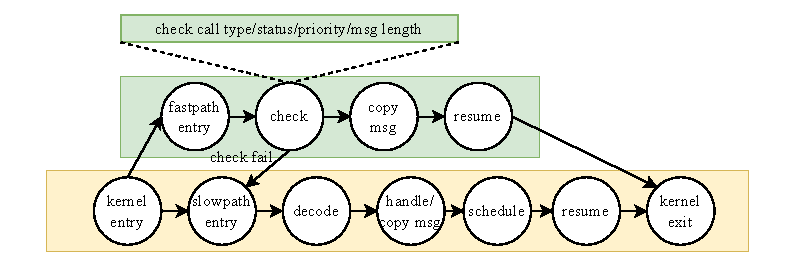
\includegraphics[width=1.0\textwidth]{figures/fast-path.drawio.pdf}
    \caption{fast-path优化示意图}\label{fig:fast-path}
\end{figure*}

在特权级切换优化方面,L4进行了多项开创性探索。虽然其物理消息寄存器方案确实降低了上下文切换开销,但前文所述的局限性最终导致该设计被虚拟寄存器方案取代\cite{heiser2016l4}。L4的其中一个创新性贡献在于发现了IPC通信中普遍存在的客户端-服务器模式特征,并据此设计了组合式系统调用接口:将Send+Reply整合为Call操作,将Reply+Recv合并为ReplyRecv操作。这种设计显著减少了特权级切换频率,至今仍是现代微内核的标准优化手段。此外,L4采用地址空间标识符(ASID)机制来缓解TLB冲刷问题,通过维护进程专属的快表项降低了上下文切换带来的性能损耗。然而,这些优化仍无法完全消除特权级切换导致的TLB污染和缓存失效问题。

除此之外,L4仅支持同步IPC,对于多核架构,同步IPC会导致服务调用被顺序执行,导致资源浪费。其次,同步IPC强制用户态以多线程的形式处理并发请求,导致了线程同步的复杂性。现代微内核在内核中引入异步通知机制,简化并发编程模型,却使得内核功能冗余,违反了内核最小化原则。

总而言之,现代微内核在单核环境下的IPC内核路径上的优化已经较为完善,在最理想的情况下仅需要两次特权级切换,然而对多核环境下,由于需要核间中断,IPC无法进入快速路径,导致多核下的IPC内核路径依旧冗长。而现代微内核在特权级切换的优化方面仍然停留缓解的层面上,导致特权级切换会成为IPC的性能瓶颈。

\subsection{特权级切换}
特权级切换带来的性能开销可分解为直接和间接两个部分。直接开销主要体现为上下文保存与恢复所需的额外指令执行周期,而间接开销则源于地址空间切换导致的缓存污染效应,这种效应会显著降低后续指令的执行效率。如表\ref{tab:seL4_call_cost}所示,基于FPGA平台的实测数据表明,在seL4微内核中执行一次Call IPC操作时,地址空间切换所产生的时间开销占比最高,其次是上下文切换和fast-path检查过程。特别值得注意的是,当fast-path检查未通过时,系统将转入slow-path处理流程,该流程涉及更复杂的消息解码和任务调度机制,会进一步加剧IPC性能的下降。针对这一关键性能瓶颈问题,学术界和工业界已从硬件架构优化和软件算法改进等多个维度展开了广泛而深入的研究探索。
\begin{table}
    \centering
    \begin{tabular}{|c|c|}
        \hline 
        操作 & 占比 \\
        \hline
        保存和恢复上下文 & 14.5\% \\
        \hline
        地址空间切换 & 59.4\% \\
        \hline
        fast - path检查 & 20.1\% \\
        \hline
        消息拷贝 & 1.5\% \\
        \hline
        其他 & 4.5\% \\
        \hline
    \end{tabular}
    \caption{seL4一次IPC中各操作的开销占比}
    \label{tab:seL4_call_cost}
\end{table}
    
从硬件出发的角度出发,大多数工作通过设计特殊的硬件或者特殊的指令来绕过内核实现IPC。如SkyBridge\cite{mi2019skybridge}允许进程在IPC中直接切换到目标进程的虚拟地址空间并调用目标函数,它通过精心设计一个Root Kernel提供虚拟化的功能,通过VMFUNC地址空间的直接切换,并通过其他一系列软件手段来保证安全性,但这种方案仅适用于虚拟化环境中。XPC\cite{du2019xpc}则直接使用硬件来提供一个无需经过内核的同步功能调用,并提供一种新的空间映射机制用于调用者与被调用者之间的零拷贝消息传递,然而该方案没有相应的硬件标准,也没有一款通用的处理器对其进行支持。这些方法都基于特殊的环境或者没有标准化的硬件来实现,适用范围有限。

从软件出发的角度出发,相关工作主要分为两类:第一类方法通过将用户态和内核态的功能扁平化来减少内核与用户态的切换开销,如unikernel\cite{kuo2020linux, olivier2019binary, yu2017web}将所有用户态代码都映射到内核态执行,Userspace Bypass\cite{zhou2023userspace} 通过动态二进制分析将两个系统调用之间的用户态代码移入内核态执行,从而减少陷入内核的次数,kernel bypass\cite{jeong2014mtcp, yang2017spdk}则通过将硬件驱动(传统内核的功能)移入用户态,从而减少上下文的切换。这些方法要么需要特殊的硬件支持,要么难以与微内核的设计理念兼容。第二类方法则是允许用户空间对多个系统调用请求排队,并通过一次提交将他们注册给内核,如FlexSC\cite{soares2010flexsc}通过在用户态设计一个用户态线程的运行时,将用户态线程发起的系统调用自动收集,然后陷入内核态进行批量执行。该方法虽然可以有效的减少陷入内核的次数,但如何设置提交的时机难以把握,过短的提交间隔将导致切换次数增加,过长的提交间隔则会导致CPU空转。

虽然现有工作难以广泛且有效地应用到微内核中,但他们的思路值得借鉴,他们的缺陷驱使研究者去寻求更好的方案。在硬件方面,一种新型的硬件技术方案——用户态中断\cite{nassif2022sapphire, RISCVPrivileged2020}逐渐被各个硬件平台(x86,RISC-V)采纳,它通过在CPU中新增中断代理机制和用户态中断的状态寄存器,当中断代理机制检测到状态寄存器发生变化时,会将中断以硬件转发的形式传递给用户态程序,从而绕过内核。该硬件方案已经在Sapphire Rapids x86处理器上和RISCV的N扩展中有了一定的支持,适用范围更加广泛。而在软件方面,异步被广泛用于请求合并和开销均摊,传统类Unix系统提供的类似select IO多路复用接口相对简陋,迫使用户态代码采用事件分发的编程范式来处理异步事件,代码相对复杂,可读性较弱。而新兴的Rust\cite{levy2015ownership, balasubramanian2017system}语言对异步有着良好的支持,其零成本抽象的设计也让它作为系统编程语言有着强大的竞争力。使用Rust进行内核和用户态基础库的开发,可以更好地对异步接口进行抽象,改善接口的易用性和代码的可读性。

\begin{table}
    \centering
    \resizebox{\textwidth}{!}{ % \textwidth 表示文本宽度,! 表示保持宽高比
    \begin{tabular}{|c|c|c|c|}
        \hline
        \textbf{优化方法} & \textbf{详细分类} & \textbf{实例} & \textbf{缺点} \\
        \hline
        \multirow{3}{*}{减少内核路径} & 临时地址映射 & [3] & \multirow{3}{*}{上下文切换开销已经成为性能瓶颈} \\
        \cline{2-3}
         & 快速路径 & \multirow{2}{*}{[3, 4, 24, 25, 26]} & \\
        \cline{2-2}
         & 消息寄存器 & & \\
        \hline
        \multirow{5}{*}{减少上下文切换开销} & 消息寄存器 & \multirow{2}{*}{[3, 4, 24, 25, 26]} & \multirow{3}{*}{无法从根本上消除切换开销} \\
        \cline{2-2} \cline{4-4}
         & 组合系统调用 & & \\
        \cline{2-3}
         & ASID机制 & [4] & \\
        \cline{2-4}
         & 统一地址空间 & [13, 14, 15, 16, 17, 18] & \multirow{2}{*}{与微内核设计理念相悖,无法有效地实施到微内核中} \\
        \cline{2-3}
         & 批量系统调用 & [19] & \\
        \hline
        \multirow{3}{*}{硬件优化} & 虚拟化指令 & [11] & 仅适用于虚拟化环境 \\
        \cline{2-4}
         & \multirow{2}{*}{直接硬件辅助} & [12] & 没有硬件标准,没有通用硬件的支持 \\
        \cline{3-4}
         & & 用户态中断 & --- \\
        \hline
        \end{tabular}
    }
    \caption{国内外研究现状汇总}
    \label{tab:optimization_methods}
\end{table}

\subsection{Rust语言与异步编程机制}
在现代计算机系统中,随着多任务处理和并发编程的普及,程序需要处理的任务越来越复杂,任务之间的依赖关系也变得越来越松散。传统的同步机制,即任务按照严格的顺序执行,前一个任务完成后才能开始后一个任务,已经无法满足高效处理多个并发任务的需求。因此,异步机制应运而生,它允许任务在不阻塞其他任务的情况下执行,从而提高了系统的整体性能和响应速度。传统操作系统大多使用C语言作为主要语言来实现异步,用于应对内核场景下的复杂场景,其虽然相对灵活,但也存在一些固有缺陷:
\begin{itemize}
    \item 编程困难:异步编程需要在代码中处理多个任务之间的协作和同步,这增加了编程的复杂性。开发者需要仔细考虑异步任务之间的依赖关系、执行顺序以及错误处理,可能导致代码难以理解和维护。
    \item 调试困难:异步编程的执行流程是非线性的,这增加了调试的难度。由于异步任务可能在不同时间点触发和执行,调试时需要跟踪多个任务的状态和交互,使得调试过程更加繁琐和耗时。
    \item 代码可读性下降:异步编程通常涉及回调函数、事件监听等结构,这些结构可能导致代码的可读性下降。回调函数的嵌套使用(即“回调地狱”)可能使代码结构变得混乱,难以阅读和理解。
    \item 代码可维护性下降:异步编程中的任务依赖关系和同步机制可能随着代码的发展而变得更加复杂,这增加了代码维护的难度。当需要修改或添加新的异步任务时,开发者需要仔细考虑对现有代码的影响,并确保新任务与现有任务之间的正确同步和协作。
  \end{itemize}

而相对高阶的语言提供了对异步的原生支持,如C++和Rust,在语言层面对异步编程提供了支持,不依赖操作系统以及标准库,有着良好的移植性和兼容性。本节我们将介绍Rust语言对异步的支持。

Rust语言的异步编程模型体现了一种系统级的创新设计,其核心思想是通过编译时状态机转换来实现高效的异步执行。该模型建立在Future这一基础抽象之上,Future trait定义的poll机制采用了一种独特的延迟执行模式,这种设计使得异步任务能够被精确控制,而非传统的事件回调模式。值得注意的是,Rust的异步机制通过编译器生成的状态机转换,在保证零成本抽象的同时,实现了与手动优化代码相当的性能表现。

在运行时支持方面,Rust采用了模块化的设计哲学。异步运行时被明确划分为Executor和Reactor两个核心组件,这种关注点分离的设计带来了显著的架构优势。Executor负责调度逻辑,而Reactor处理I/O事件通知,二者的协同工作通过高效的wake机制实现。特别值得关注的是,Rust的标准库刻意不绑定特定的运行时实现,这种设计决策赋予了开发者根据应用场景选择最优运行时的灵活性。从系统编程的角度看,这种模块化设计使得异步Rust能够适应从嵌入式系统到分布式服务的各种应用场景。

语言层面的async/await语法为异步编程提供了重要的工程实践支持。这一语法糖不仅大幅提升了代码的可读性和可维护性,更重要的是,它使得编译器能够进行深度的优化。通过将异步控制流转换为状态机,Rust实现了与手动编写回调代码相当的性能,同时避免了回调地狱等常见的异步编程陷阱。从类型系统的角度来看,async函数返回的Future保持了严格的类型约束,这使得编译器能够在编译期捕获大量潜在的逻辑错误,显著提升了异步代码的可靠性。

此外,Rust语言的设计哲学与微内核架构在系统安全性和可靠性方面展现出深刻的协同效应。从内存管理机制来看,Rust的所有权系统通过编译时的严格检查,为微内核的关键组件提供了静态的内存安全保障。这种编译期验证机制与微内核最小化特权域的设计原则高度契合,使得内核开发者能够在保证性能的前提下,有效预防各类内存安全漏洞。

基于上述工程实践考量,本文选择Rust作为ReL4微内核的主要实现语言。这一选择不仅能够充分利用Rust在系统编程领域的独特优势,更重要的是,Rust的现代化语言特性为构建安全、高效的异步微内核提供了更加理想的开发工具链。

\subsection{用户态中断与TAIC加速器}

现代处理器通过多特权级设计实现安全隔离,但特权级切换带来的性能开销已成为系统优化的关键瓶颈。传统的中断处理机制依赖于内核介入,导致频繁的特权级切换和上下文保存恢复操作,不仅产生直接的指令执行开销,还会因页表切换和缓存失效引入显著的间接性能损失。

\begin{figure*}[htbp]
    \centering
    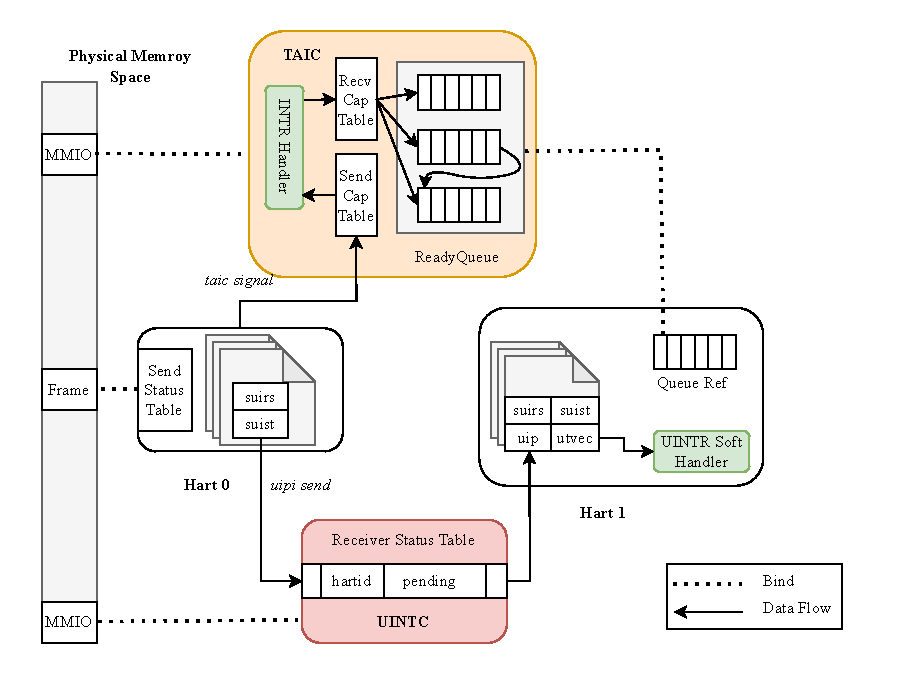
\includegraphics[width=1.0\textwidth]{figures/uintc_taic.drawio.pdf}
    \caption{用户态中断和TAIC加速器的示意图}\label{fig:uintc_taic}
\end{figure*}

为降低这一开销,用户态中断(User-Level Interrupt)机制应运而生。该技术通过在CPU中引入中断代理和专用状态寄存器,使中断能够直接在用户态处理,完全绕过内核参与。以RISC-V N扩展的实现为例,如\ref{fig:uintc_taic}所示,用户态中断的核心创新在于将中断状态管理分为操作系统维护的发送状态表和硬件控制器(UINTC)管理的接收状态表。当触发中断时,硬件通过专用指令自动完成状态查询和处理器间中断传递,最终直接跳转到用户态注册的处理函数执行。这一设计不仅消除了内核转发的软件开销,还保持了良好的缓存局部性。


在UINTC基础上的进一步优化催生了任务感知中断控制器(TAIC)。与基础用户态中断相比,TAIC的创新性体现在两个方面:首先,它将所有状态表统一交由硬件管理,通过MMIO寄存器访问替代内存查表操作,减少了中断发送阶段的内存访问延迟;其次,该控制器深度整合了任务调度功能,能够在中断到达时自动将预注册的处理任务加入硬件就绪队列,完全消除了软件唤醒的开销。这种硬件-软件协同设计使得中断处理流程更加高效,在保持用户态执行优势的同时,进一步减少了CPU执行流的打断频率,为实时性要求高的应用场景提供了更优的解决方案。

从系统架构演进的角度看,从传统内核中断到用户态中断,再到任务感知中断控制器的发展,体现了中断处理机制从软件主导到硬件加速的转变趋势。这种转变不仅降低了中断延迟,更重要的是通过硬件原语支持,为构建更高效的异步任务处理框架奠定了基础。


\section{主要研究内容}
本文以免费开源的seL4的IPC系统主要研究对象,介绍了seL4中IPC的设计细节以及相关设计缺陷,针对seL4的相关缺陷,基于用户态中断,给出了高性能异步微内核的整体设计方案,包含了无需内核转发的通知机制U-notification、异步IPC与异步系统调用,并基于Rust语言在RISC-V平台实现了ReL4原型系统。在FPGA上将U-notification、异步IPC 和异步系统调用分别与seL4进行了对比测试,并评估了ReL4在真实的TCP Server Benchmark上的性能表现。论文内容结构安排如下:

第1章,绪论部分,阐述了本课题的研究背景及意义,国内外研究现状和发展趋势,最后概述了本课题的研究内容和对内容的组织结构。

第2章,介绍了seL4系统的发展历史和主要特征,并对seL4中的基本概念以及IPC设计进行了系统性阐述。

第3章,系统设计部分。首先介绍了ReL4与seL4的关系,ReL4的特点以及设计目标,然后介绍了ReL4如何对系统中各个部分的通知机制进行支持和优化,最后介绍了用于保证兼容性和提升易用性的异步运行时的组成部分和设计思路。

第4章,系统实现部分。主要介绍了新增的系统调用,以及基于U-notification的异步运行时如何实现异步IPC和异步系统调用,并讨论了ReL4在通知机制、IPC机制和系统调用中对seL4的兼容程度。

第5章,系统评估部分。首先介绍了ReL4的测试方案,然后针对ReL4的各个机制进行了性能评估和分析,最后测试了ReL4在真实的TCP Server Benchmark上的性能表现。

第6章,总结与展望,对本次设计和论文工作进行了总结,并提出了进一步的研究方向与对未来工作的展望。